\documentclass[a4paper,12pt]{report}
\usepackage[utf8]{inputenc}
\usepackage[francais]{babel}
\usepackage{fancyhdr}
\usepackage{graphicx}
\usepackage{tikz}
\usetikzlibrary{calc}
\usepackage{listings}
\usepackage{xcolor}
\definecolor{grey}{rgb}{0.9,0.9,0.9}
\usepackage{titlesec}
\usepackage{verbatim}
\usepackage{listings}
\usepackage{textcomp}
\usepackage{hyperref}
\usepackage{longtable}
\usepackage{colortbl}
\usepackage{amssymb}


\frenchbsetup{StandardLists=true}
\newcommand{\marge}{18mm}
\usepackage[left=\marge,right=\marge,top=\marge,bottom=\marge]{geometry}
\pagestyle{fancy}
\setlength{\headheight}{14pt}
\chead{
  \textbf{Binôme :} Douaille Erwan \& Yanis Nait Abdelaziz
  \hspace{2em}
  \textbf{Groupe :} M1 Info TI}
\renewcommand{\headrulewidth}{1pt}
\linespread{1}
\setlength{\columnseprule}{0.2pt}
\definecolor{javakeyword}{rgb}{0,0,0.5}
\definecolor{javastring}{rgb}{0,0.5,0}
\definecolor{javacomment}{rgb}{0.5,0.5,0.5}
\lstdefinestyle{java}{
   language=Java, basicstyle=\footnotesize,       % the size of the fonts that are used for the code
  numbers=left,                   % where to put the line-numbers
  numberstyle=\tiny\color{gray},  % the style that is used for the line-numbers
  stepnumber=1,                   % the step between two line-numbers. If it's 1, each line
                                  % will be numbered
  numbersep=5pt,                  % how far the line-numbers are from the code
  backgroundcolor=\color{white},  % choose the background color. You must add \usepackage{color}
  showspaces=false,               % show spaces adding particular underscores
  showstringspaces=false,         % underline spaces within strings
  showtabs=false,                 % show tabs within strings adding particular underscores
  frame=single,                   % adds a frame around the code
  rulecolor=\color{black},        % if not set, the frame-color may be changed on line-breaks within not-black text (e.g. commens (green here))
  tabsize=2,                      % sets default tabsize to 2 spaces
  captionpos=b,                   % sets the caption-position to bottom
  breaklines=true,                % sets automatic line breaking
  breakatwhitespace=false,        % sets if automatic breaks should only happen at whitespace
  title=\lstname,                 % show the filename of files included with \lstinputlisting;
   stringstyle=\color{javastring},
   keywordstyle=\color{javakeyword}\ttfamily\textbf,
   commentstyle=\color{javacomment}\ttfamily\textit
 }

\begin{document}



\makeatletter
\begin{titlepage}
\centering
\vspace{-10em}
{\LARGE \textbf{\textsc{Rapport de Projet RVI}}}\\
\vspace{3em}

\includegraphics[scale=0.6]{image/thalassa.png}\\
\vspace{3em}
{\LARGE \textsc{Projet Thalassa: simulation de plongée sous-marine}}\\

\vspace{8em}
Par\\
\vspace{1em}
{\LARGE \@author}\\

\vspace{2em}



\begin{tikzpicture}[remember picture,overlay]

\node [below left,xshift=-1cm, yshift=4cm] at (current page.south east){
\includegraphics[scale=0.6]{image/ustl1.png}};

\end{tikzpicture}
\end{titlepage}
\makeatother

\sloppy

\setcounter{page}{1} 
\newpage

\section*{Introduction}

Dans ce tp, nous allons travailler les fréquences spatiales qui subiront l'effet de moiré lors d'un sous-échantillonage. Nous verrons comment maîtriser cet effet en appliquant des corrections sur les images résultantes du sous-échantillonage.


\section*{Question 1}

\begin{figure}[!ht]
	\center	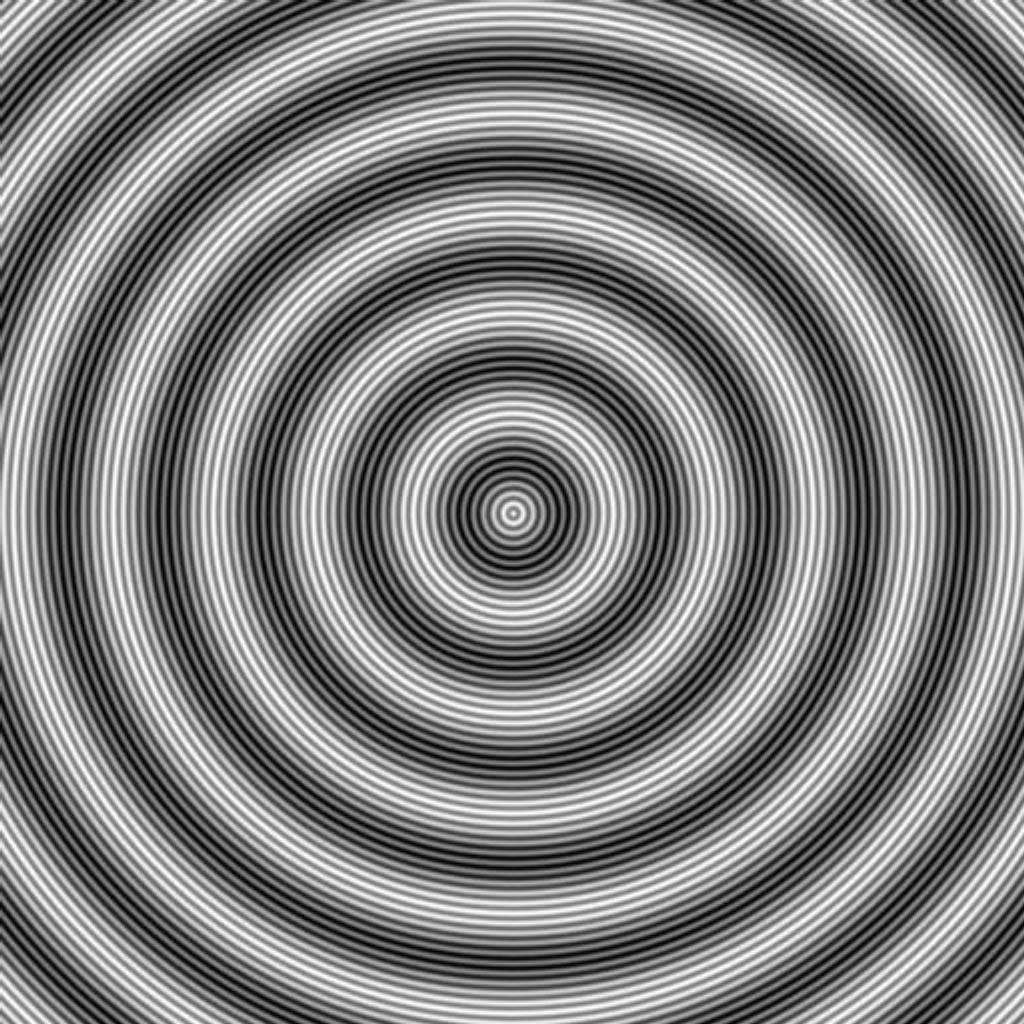
\includegraphics[scale=0.15]{image/1024_moire.jpg}	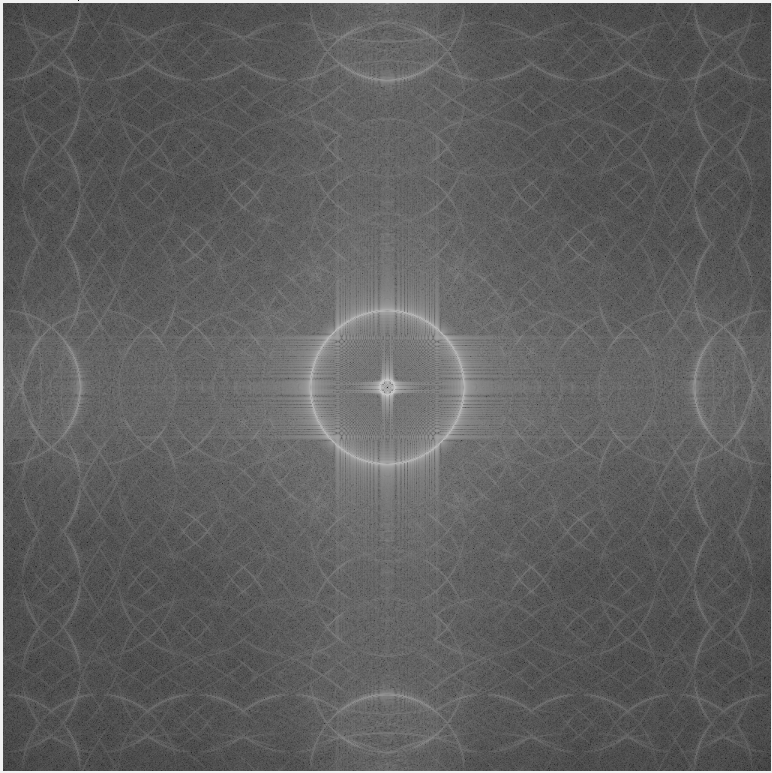
\includegraphics[scale=0.2]{image/q1_FFT_original.png}
	\caption{Image original avec la résultante de la FFT}
\end{figure}


Dans l'image de droite, qui est le résultat de la tranformé de fourier sur l'image originale, on observe 2 grands cercles. Le cercle central représente les basses féréquences et le plus grand, les hautes fréquences.

\begin{figure}[!ht]
	\center	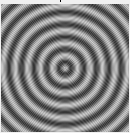
\includegraphics[scale=1]{image/q1_scale.png}	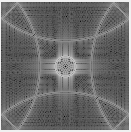
\includegraphics[scale=1]{image/q1_FFT_scale.png}
	\caption{Image scalé avec la résultante de la FFT}
\end{figure} 

L'image correspondant à la transformée de fourier de l'image sous-échantillonée fait apparaître des demi-cercles représentant les cercles visibles dans la FFT de l'image originale.

\newpage

\section*{Question 2}

\begin{figure}[!ht]
	\center	
		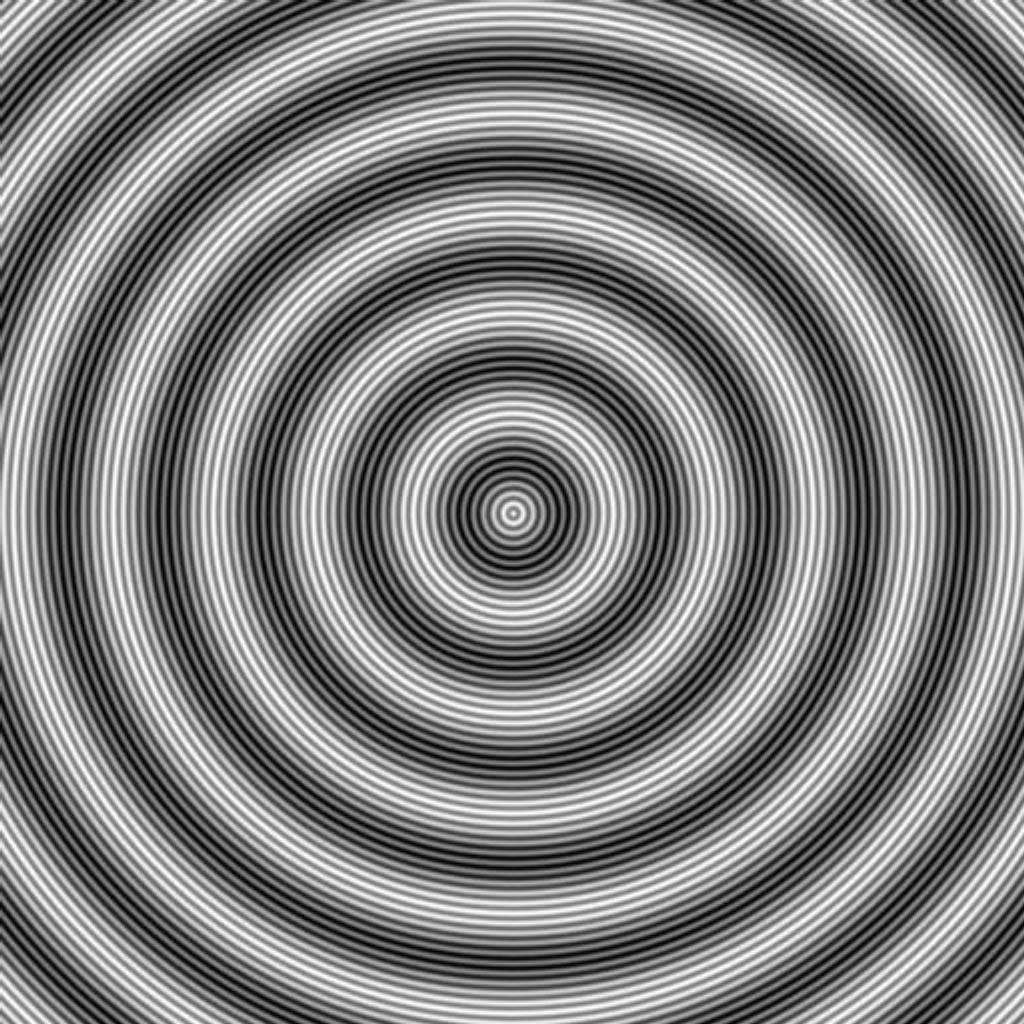
\includegraphics[scale=0.1]{image/1024_moire.jpg}		
		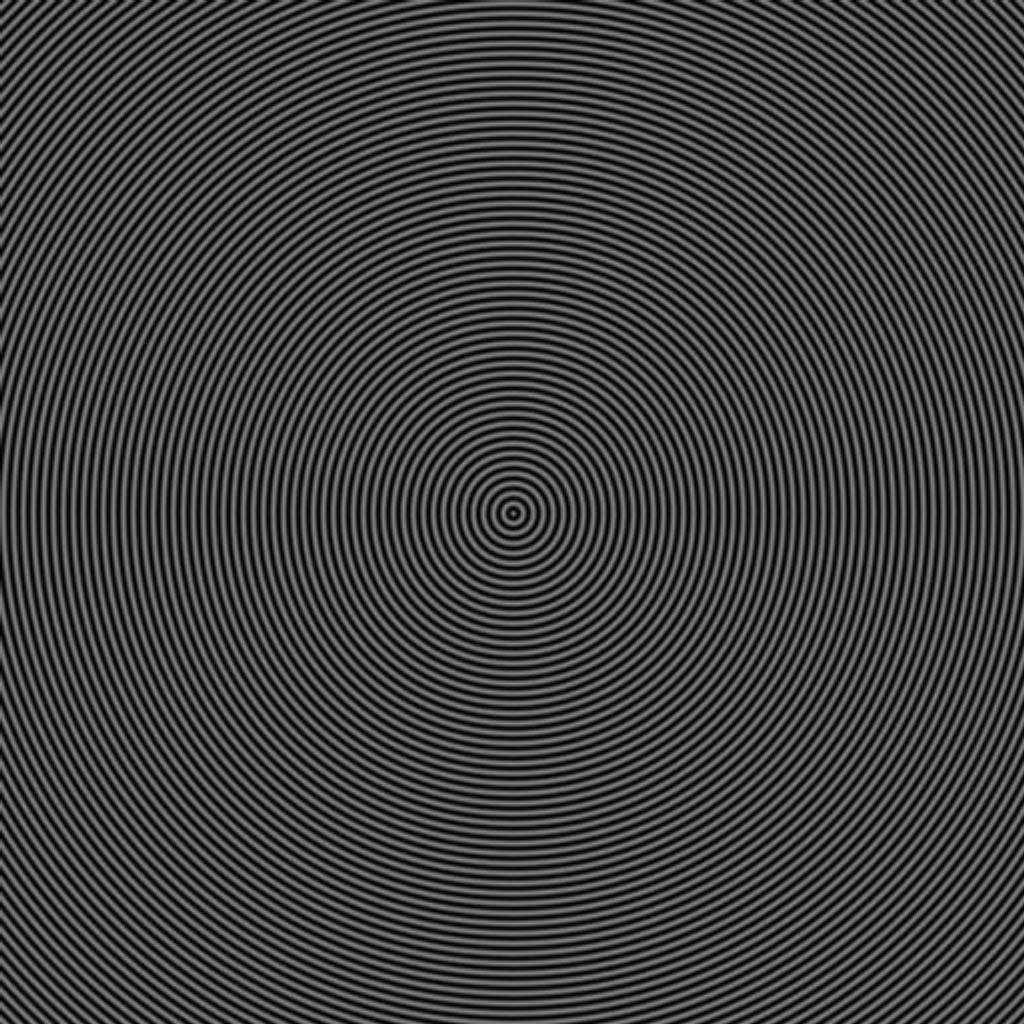
\includegraphics[scale=0.1]{image/1024_moire_f1.jpg}	
		
\includegraphics[scale=0.1]{image/1024_moire_f2.png}	
\end{figure}
Une fois les images \textit{1024$\_$moire$\_$f1.jpg} et \textit{1024$\_$moire$\_$f2.tif} additionnées nous obtenons l'image \textit{1024$\_$moire.jpg}.

L'image originale est une superposition de \textit{1024$\_$moire$\_$f1.jpg} et \textit{1024$\_$moire$\_$f2.tif}

On peut donc en conclure que nous pouvons obtenir  \textit{1024$\_$moire$\_$f1.jpg} par soustraction de  \textit{1024$\_$moire.jpg} par \textit{1024$\_$moire$\_$f2.tif}.

\section*{Question 3}

\begin{lstlisting}[float,style=Java,caption={Code question 3 et 4},label=lst:question34]
distance = sqrt(pow(i_max_2 - i_max_1, 2) + pow(j_max_2 - j_max_1, 2));
if(i_max_1!=i_max_2 && j_max_1!=j_max_2){
	print("texture diagonale");
} else if(i_max_1==i_max_2 && j_max_1!=j_max_2){
	print("texture verticale");
} else if(i_max_1!=i_max_2 && j_max_1==j_max_2){
	print("texture horizontal");
}
omega=distance/sqrt(W*H);
print("omega=",omega);
\end{lstlisting}

\begin{figure}[!ht]
	\center	
		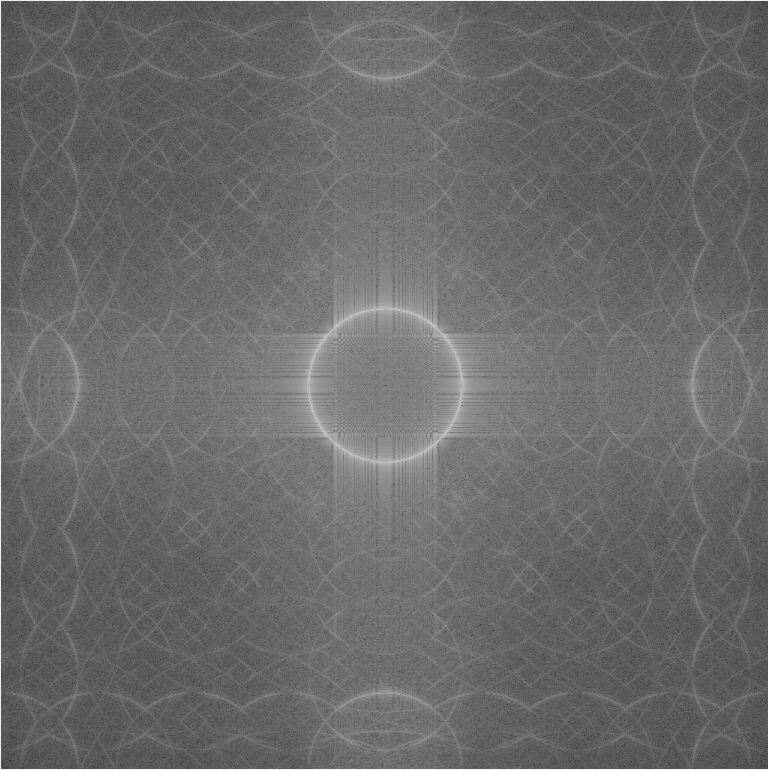
\includegraphics[scale=0.1]{image/q3.png}		
\end{figure}
Nous obtenons les fréquences spatiales grâce au code obtenus dans le précédent tp, voir le code ci-dessus.

La fréquence spatiale $\omega$ $_{1}$ = 0.1002

\newpage

\section*{Question 4}

\begin{figure}[!ht]
	\center	
		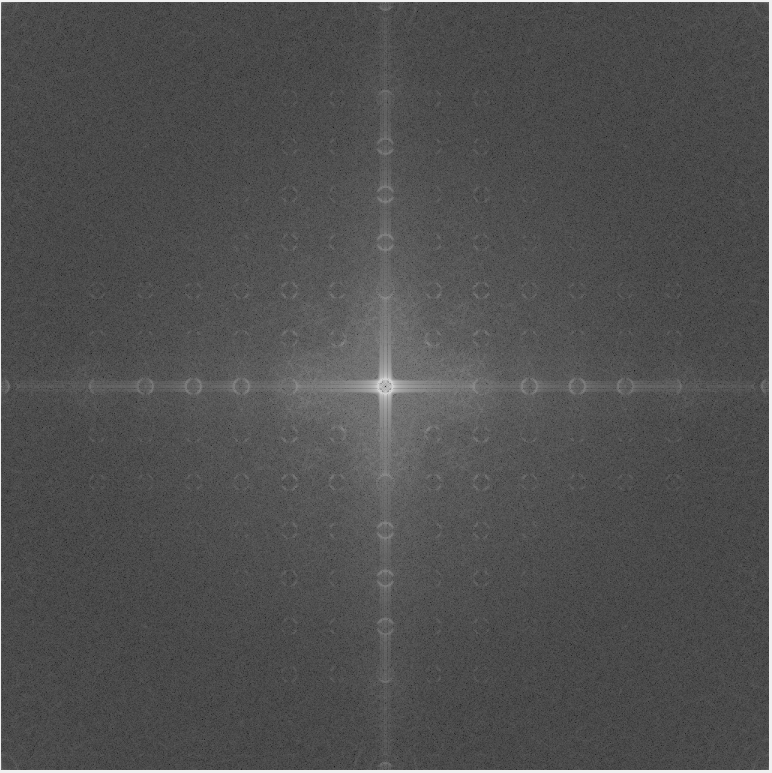
\includegraphics[scale=0.1]{image/Q4.png}	
\end{figure}
La fréquence spatiale $\omega$ $_{1}$ = 0.01038


\section*{Question 5}


\begin{figure}[!ht]
	\center	
		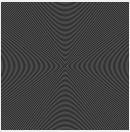
\includegraphics[scale=1]{image/q5_f1.png}	
		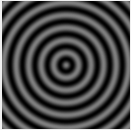
\includegraphics[scale=1]{image/q5_f2.png}	
\end{figure}

On observe que l'effet de moiré apparaît sur l'image \textit{1024$\_$moire$\_$f1.png} et non sur \textit{1024$\_$moire$\_$f2.png}. On peut donc en conclure que plus les fréquences sont hautes plus l'effet de moiré apparaîtra sur les images sous-échantillonées.

\section*{Question 6}

Nous savons que pour une image sous-échantilloné la fréquence d'un motif cycle doit être supérieur à 0,5 cycle/pixel pour obtenir l'effet de moiré. Afin d'empêcher l'effet de moiré dans une image sous-échantillonée d'un facteur 8, l'image originale doit avoir une fréquence spatiale inféreieure à 0,5/8 soit 0.0625.

\section*{Question 7}

On sait que pour une fréquence spatiale inférieure à 0.0625 l'image ne subira pas l'effet de moiré, donc à partir de cette observation on peut dire que $\omega$ $_{2}$ évite le phénomène de repliement de spectre au sein de l'image sous-échantillonée.

\section*{Question 8}

Pour une image obtenue par superposition des basses et des hautes fréquences, sa fréquence sera égale à la haute fréquence. Donc dans l'image sous échantillonée les basses fréquences ne changent pas tandis que les hautes fréquences seront multipliées par le facteur de sous-échantillonage.


\section*{Question 9}


\newpage

%%%%%%%%%%%%%%%%%%%%%%%%%%%%%%%%%%%%%%%%%% CONCLU
%%%%%%%%%%%%%%%%%%%%%%%%%%%%%%%%%%%%%%%%%%%%%%%%%
%%%%%%%%%%%%%%%%%%%%%%%%%%%%%%%%%%%%%%%%%%%%%%%%%
\section*{Conclusion}
Dans ce tp , nous avons pu comprendre comment l'effet de moiré apparaît, comment l'éviter et le corriger. L'effet de moiré apparaît sur les images contenant des motifs cycle de haute fréquence et non de basse fréquence. Nous avons également pu déterminer à partir de quel valeur une fréquence spatiale subira l'effet de moiré. La correction de l'effet de moiré se réalise en appliquant ?. 
\end{document}